\documentclass[11pt,a4paper]{article}
% ---------- page and fonts (matched to the AI651 handout) ----------
\usepackage[margin=1in]{geometry}
\usepackage[T1]{fontenc}
\usepackage{lmodern}                 % Computer Modern, as in the handout
\usepackage{amsmath,amssymb}
\usepackage{graphicx}
\usepackage{booktabs}
\usepackage{float}
\usepackage{xcolor}
\usepackage{enumitem}
\usepackage[skip=8pt plus 2pt]{parskip}   % no indent, space between paragraphs
\usepackage{titlesec}
\usepackage[most]{tcolorbox}
\usepackage{hyperref}

% ---------- handout colours ----------
\definecolor{headteal}{RGB}{21,94,117}   % section headings
\definecolor{boxnavy}{RGB}{20,60,110}    % box title bar
\definecolor{boxgray}{RGB}{243,244,246}  % box body
\hypersetup{colorlinks=true,linkcolor=headteal,urlcolor=headteal,citecolor=headteal}

% ---------- heading style: bold serif in teal ----------
\titleformat{\section}{\color{headteal}\Large\bfseries}{\thesection.}{0.8em}{}
\titleformat{\subsection}{\color{headteal}\large\bfseries}{\thesubsection.}{0.8em}{}
\titleformat{\subsubsection}{\color{headteal}\normalsize\bfseries}{\thesubsubsection.}{0.8em}{}
\titlespacing*{\section}{0pt}{14pt}{8pt}
\titlespacing*{\subsection}{0pt}{12pt}{6pt}
\titlespacing*{\subsubsection}{0pt}{10pt}{4pt}

% ---------- handout-style box (navy title bar, grey body) ----------
\newtcolorbox{infobox}[1]{enhanced,colback=boxgray,colframe=boxnavy,
  coltitle=white,fonttitle=\bfseries\small,title={#1},
  boxrule=0.6pt,arc=1.5pt,left=6pt,right=6pt,top=4pt,bottom=4pt}

\setlist{nosep,leftmargin=1.4em}

% ---------- helpers ----------
% \todo{...} marks text still to write (red, easy to spot; delete all before submitting)
\newcommand{\todo}[1]{\textcolor{red}{[TODO: #1]}}
\newcommand{\figph}[2]{%
  \begin{figure}[H]\centering
  \fbox{\parbox[c][4cm][c]{0.85\linewidth}{\centering\textcolor{gray}{Figure placeholder: \detokenize{#1}}}}
  \caption{#2}\label{fig:#1}\end{figure}}

\begin{document}

% =====================================================================
\thispagestyle{empty}
\begin{center}
\textbf{Lahore University of Management Sciences}\\
Syed Babar Ali School of Science and Engineering (SBASSE)\\
\textbf{AI651 -- Deep Learning for Space, Time and Graphs}\\
Fall 2026\\[6pt]
\textbf{Assignment 1 -- Report}
\end{center}

\noindent\rule{\linewidth}{0.6pt}\\[2pt]
\textbf{Name:} Hasan Amjad \hfill \textbf{Roll No.:} 25280042\\[2pt]
\textbf{GitHub repository:} \url{https://github.com/HasanAmjad/autoformer-exogenous-forecasting}\\[-4pt]
\noindent\rule{\linewidth}{0.6pt}

\vspace{6pt}
\begin{infobox}{Contents of submission}
This report (PDF and \LaTeX\ source); the executed \texttt{PA1\_PRESET=full} Task~1 notebook;
each numbered figure as a PDF; Task~2 code and notebooks (\texttt{v1}, \texttt{v2}, \texttt{v3} and \texttt{analysis}) in the repository.
\end{infobox}

\clearpage

% =====================================================================
\section*{Task 1 -- Forecasting Across Heterogeneous Sensors}
\addcontentsline{toc}{section}{Task 1}

\begin{infobox}{Run configuration}
Preset \texttt{full}; data seed 0; model seed 0; device \texttt{mps} (Apple GPU);
eligible train/validation/test origins 650/105/105.
All numbers below come from this single full run. Unless stated otherwise, errors are
\textbf{validation} RMSE in m/s$^2$; ``established'' = Stations 1--3, ``held-out'' = Station~4.
\end{infobox}

% ---------------------------------------------------------------------
\subsection*{Response 1A -- Predicted vs.\ measured ordering}

My prediction prior to running Output 1.1 was as follows:

\begin{table}[H]\centering\small
\caption{Predicted ordering, written before running Output 1.1.}
\label{tab:pred1a}
\begin{tabular}{ll}
\toprule
Population & Prediction (best $\to$ worst)\\
\midrule
Established stations & Raw Attention $>$ Period-routed $>$ Shared $>$ Sensor-specific\\
Station 4 forecast   & Raw Attention $>$ Period-routed $>$ Shared ridge\\
\bottomrule
\end{tabular}
\end{table}

Sensor-specific ridge isn't part of the Station~4 forecast, since it requires a matrix fitted on that station's own training data, which isn't available in our case because Station~4 is held out. My intuition for why Raw Attention may lead was that it is basically a neural network that builds its own mixing rule from each window. It can handle changing data because its attention weights are recomputed from the current window, so the same learned projections produce a different mixing rule for each operating speed.

\begin{table}[H]\centering\small
\caption{Output 1.1 -- validation RMSE (m/s$^2$) by population and product.}
\label{tab:out11}
\begin{tabular}{lcccccccc}
\toprule
 & \multicolumn{4}{c}{Established (Stations 1--3)} & \multicolumn{4}{c}{Held-out (Station 4)}\\
\cmidrule(lr){2-5}\cmidrule(lr){6-9}
Model & All & A & B & C & All & A & B & C\\
\midrule
Shared ridge          & 0.767 & 0.805 & 0.854 & 0.621 & 0.876 & 0.909 & 0.982 & 0.713\\
Sensor-specific ridge & 0.768 & 0.804 & 0.852 & 0.630 & n/a & n/a & n/a & n/a\\
Period-routed ridge   & \textbf{0.166} & \textbf{0.181} & \textbf{0.164} & \textbf{0.152} & \textbf{0.173} & \textbf{0.184} & \textbf{0.182} & \textbf{0.150}\\
Raw Attention         & 0.436 & 0.412 & 0.462 & 0.433 & 0.659 & 0.677 & 0.619 & 0.678\\
\bottomrule
\end{tabular}
\end{table}

The measured output (Table~\ref{tab:out11}) tells a different story: Period-routed ridge and Raw Attention swap places in both the established and Station~4 forecasts. On established stations, Period-routed ridge reaches an RMSE of 0.166 against 0.436 for Raw Attention; on Station~4 it is 0.173 against 0.659. As anticipated, errors get worse when moving to the held-out Station~4, and the trend is similar in both cases, though it gets much worse for Raw Attention (0.436 $\to$ 0.659, +51\%) compared with Period-routed ridge (0.166 $\to$ 0.173, +4\%) and Shared ridge (0.767 $\to$ 0.876, +14\%).

The RMSE for Period-routed ridge is the lowest because it conditions on exactly the quantity that changes, the period. Within one speed band, continuing the wave is nearly a linear operation, so once a person has supplied the right variable, a small closed-form model is enough. Raw Attention didn't do as well as I initially thought because it has to learn this speed dependence from the data on its own. Meanwhile, the slow drift dominates the raw input, and every pair of positions is scored separately instead of being grouped by their spacing. Its large drop on Station~4 also suggests it partly learned station-specific details rather than the speed structure.

Shared and Sensor-specific ridge have practically the same RMSE on established stations (0.767 vs.\ 0.768). The reason is that the underlying forecasting rule depends on the machine's speed, not on which station produced the data. Splitting by station just leaves each formula with less data, and each one still has to average across speeds.

\paragraph{Revised ordering (both populations).}
\textbf{Period-routed ridge $>$ Raw Attention $>$ Shared ridge $\approx$ Sensor-specific ridge} (the last is unavailable for Station~4).

% ---------------------------------------------------------------------
\subsection*{Response 1B -- Why the forecasting rule must depend on context}

\begin{figure}[H]\centering
\includegraphics[width=0.92\linewidth]{{figures/1.2-1}.pdf}
\caption{Output 1.2 -- Station 1 under Product A ($P\approx16.1$) and Product C ($P\approx30.1$).}
\label{fig:out12}
\end{figure}

The single matrix $\widehat W$ in Eq.~(8) is fitted by least squares over \emph{all} training windows, which mix periods from 14 to 36 samples. A 16-sample cycle and a 30-sample cycle need different phase advances over the same 48-step horizon, so one fixed operator can only return their least-squares compromise. In Figure~\ref{fig:out12} this compromise is visible as \textbf{amplitude shrinkage and phase lag}: for Product~A the shared and sensor-specific ridge forecasts have visibly flattened peaks and fall behind the true oscillation in the second half of the horizon (window RMSE 0.779 and 0.787), while period-routed ridge, which uses a matrix fitted only to similar paces, tracks it (0.232). Averaging continuations whose phases disagree partly cancels them, which is why the compromise forecast is damped rather than simply shifted.

\begin{figure}[H]\centering
\includegraphics[width=\linewidth]{{figures/1.3-1}.pdf}
\caption{Output 1.3 -- Attention maps for two Station 1 contexts and their difference.}
\label{fig:out13}
\end{figure}

Attention uses the \emph{same} learned $W_Q, W_K, W_V$ for both contexts, but its scores $QK^\top/\sqrt{d_h}$ are computed from the current window. Different inputs therefore give different weight matrices: in Figure~\ref{fig:out13} the Product~A and Product~C maps concentrate on different key positions, with a mean absolute weight difference of 0.013 and a maximum of 0.284. Each context thus receives its own value-mixing operation, whereas ridge applies the identical $\widehat W$ to every window. (This only shows that the mixing is context-dependent; it is not evidence that the attention weights have recovered the physical period.)

% ---------------------------------------------------------------------
\subsection*{Response 2 -- Separating slow structure from repetition}

\begin{figure}[H]\centering
\includegraphics[width=\linewidth]{{figures/2.1-1}.pdf}
\caption{Output 2.1 -- trend and remainder for candidate widths (Station 2, Product C).}
\label{fig:out21}
\end{figure}

\begin{figure}[H]\centering
\includegraphics[width=0.6\linewidth]{{figures/2.2-1}.pdf}
\caption{Output 2.2 -- oracle period recovery (training data only).}
\label{fig:out22}
\end{figure}

\begin{table}[H]\centering\small
\caption{Outputs 2.1--2.2 -- effect of the averaging width $m$.}
\label{tab:out22}
\begin{tabular}{lccccc}
\toprule
 & raw & $m=17$ & $m=25$ & $m=33$ & $m=41$\\
\midrule
Remainder std (m/s$^2$) & -- & 0.578 & 1.012 & 1.372 & 1.572\\
Oracle recovery within one sample & 0.687 & 0.980 & 0.989 & 0.993 & \textbf{0.998}\\
Median period error (samples) & 0.525 & 0.157 & 0.122 & 0.142 & 0.216\\
\bottomrule
\end{tabular}
\end{table}

\begin{table}[H]\centering\small
\caption{Output 2.3 -- decomposition ablation, validation RMSE (m/s$^2$).}
\label{tab:out23}
\begin{tabular}{lcccc}
\toprule
Model & Established & Held-out & Est.\ A / B / C & Held-out A / B / C\\
\midrule
Raw Attention & 0.436 & 0.659 & 0.412 / 0.462 / 0.433 & 0.677 / 0.619 / 0.678\\
Attention + decomposition & \textbf{0.324} & \textbf{0.486} & 0.302 / 0.375 / 0.289 & 0.428 / 0.556 / 0.464\\
\bottomrule
\end{tabular}
\end{table}

\begin{itemize}
  \item \textbf{Selected width $m=41$.} Visually (Fig.~\ref{fig:out21}), narrow widths let the trend follow part of the vibration: at $m=17$ the trend wiggles and the remainder is weak (std 0.578). As $m$ grows the trend becomes a smooth ramp and the remainder becomes a clean, full-amplitude oscillation (std 1.572 at $m=41$); after decomposition the period score peaks sharply at the true period (32), while the raw context gives almost no peak. Empirically, oracle period recovery rises from 0.687 (raw) to 0.998 ($m=41$), and in Output 2.3 adding decomposition to Attention lowers validation RMSE by \textbf{26\%} on established stations (0.436 $\to$ 0.324) and by \textbf{26\%} on Station~4 (0.659 $\to$ 0.486), improving every product.
  \item \textbf{Why a moving average suits this world.} The drift varies on a 240-sample scale while the vibration has periods of 14--36 samples. A 41-sample window is longer than every vibration period, so it averages each cycle to approximately zero, yet it is much shorter than 240, so the drift passes into the trend almost unchanged. The training-only oracle diagnostic is a sound way to choose $m$ because it directly measures the property we want (does the remainder expose the true repetition?) using information available only in the synthetic training data, without touching validation or test data. Note that the selection criterion matters: $m=41$ maximises recovery within one sample, while $m=25$ has the smallest median period error.
  \item \textbf{Where it fails / alternative.} A fixed moving average fails at an \emph{abrupt level shift} (e.g.\ a product changeover or impact inside the window): it smears the step over 41 samples and leaks a spurious transient into the remainder. It would also fail if a vibration period exceeded the window. An alternative is \textbf{STL/LOESS decomposition}, which fits local polynomials and assumes a locally smooth (curved) trend rather than a locally constant one, at the cost of more computation and tuning.
\end{itemize}

\begin{figure}[H]\centering
\includegraphics[width=0.92\linewidth]{{figures/2.3-1}.pdf}
\caption{Output 2.3 -- largest and smallest decomposition gains (Station 4).}
\label{fig:out23}
\end{figure}

% ---------------------------------------------------------------------
\subsection*{Response 3 -- Mixing by temporal delay}

\noindent Implementation check: \texttt{aggregate\_delays} reproduces the worked example
(35, 15, 25, 25, so $z_0=35$ and the shift runs the right way) and passes the gradient check; Output 3.1 confirms \texttt{delay\_scores} against a direct circular correlation (4, $-4$, 4, $-4$).

\begin{figure}[H]\centering
\includegraphics[width=\linewidth]{{figures/3.2-1}.pdf}
\caption{Output 3.2 -- signal-level recurrence diagnostic (Station 2, Product A, $P\approx16.1$). This is a correlation computed directly from the signal, not the model's learned q/k scores.}
\label{fig:out32}
\end{figure}

\begin{itemize}
  \item \textbf{Strongest lags.} The residual correlation peaks at lag \textbf{16} (0.896) and lag \textbf{32} (0.897), i.e.\ at the run's period $P\approx16.1$ and its multiple $2P\approx32.3$; the troughs at about 8, 24 and 40 samples are the half-period offsets, where peaks align with troughs.
  \item \textbf{Why decomposition cleans the evidence.} In the raw signal the correlation simply decays from about 0.45 at lag 8 to $-0.55$ at lag 40, with no peak at $P$: the slow ramp is similar to itself at every small shift and dominates the score. Removing the trend leaves an almost pure oscillation, so peaks align only at multiples of $P$. This supports the delay mixer's inductive bias: if useful information sits at a few recurring displacements, scoring $L$ delays (instead of $L^2$ position pairs) and aggregating shifted copies is the natural mechanism, and it works best on the decomposed stream. Consistently, in Output 4.1 the delay mixer alone already halves Raw Attention's error (0.436 $\to$ 0.214).
  \item \textbf{Where delay mixing is the wrong bias.} An \emph{isolated transient}, such as a single impact from a loose part, has no recurring displacement. The delay mixer would either average it away or copy it forward at the selected lags as false ``echoes'', because it can only reuse shifted copies of the context. Similarly, if the period drifts quickly within one context (machine run-up), no small fixed set of lags aligns the whole window.
\end{itemize}

% ---------------------------------------------------------------------
\subsection*{Response 4 -- Comparing designs and deploying}

\paragraph{(a) Prediction (written before Output 4.1).}
I expect decomposition to help most, since it splits off the slow trend with a moving average and sends it to a simple linear head, leaving the encoder only the faster vibration.

\paragraph{(b) Validation results (Outputs 4.1--4.2).}
\begin{table}[H]\centering\small
\caption{Validation error by model. RMSE in m/s$^2$, MSE in (m/s$^2$)$^2$.}
\label{tab:out41}
\begin{tabular}{lcccccc}
\toprule
 & \multicolumn{2}{c}{Established} & \multicolumn{2}{c}{Held-out} & & \\
\cmidrule(lr){2-3}\cmidrule(lr){4-5}
Model & RMSE & MSE & RMSE & MSE & Params & Fit (s)\\
\midrule
Shared ridge & 0.767 & 0.588 & 0.876 & 0.767 & 4{,}608 & 0.001\\
Sensor-specific ridge & 0.768 & 0.590 & n/a & n/a & 13{,}824 & 0.001\\
Period-routed ridge & \textbf{0.166} & \textbf{0.028} & \textbf{0.173} & \textbf{0.030} & 59{,}904 & 0.002\\
\midrule
Raw Attention & 0.436 & 0.190 & 0.659 & 0.434 & 368{,}368 & 206\\
Attention + decomposition & 0.324 & 0.105 & 0.486 & 0.236 & 373{,}024 & 292\\
Raw delay mixer & 0.214 & 0.046 & 0.338 & 0.114 & 368{,}370 & 776\\
Autoformer-inspired & 0.197 & 0.039 & 0.244 & 0.059 & 373{,}026 & 852\\
\bottomrule
\end{tabular}
\end{table}

\begin{figure}[H]\centering
\includegraphics[width=0.92\linewidth]{{figures/4.1-1}.pdf}
\caption{Output 4.1 -- contrasting forecast cases for the four neural configurations.}
\label{fig:out41}
\end{figure}

\begin{figure}[H]\centering
\includegraphics[width=\linewidth]{{figures/4.2-1}.pdf}
\caption{Output 4.2 -- validation RMSE across the 48-step horizon.}
\label{fig:out42}
\end{figure}

\paragraph{Interpretation ($\le$ 200 words).}
On established stations, decomposition alone lowers Raw Attention's RMSE from 0.436 to 0.324 ($-26\%$), delay mixing alone to 0.214 ($-51\%$), and both together to 0.197 ($-55\%$). The gains are \textbf{sub-additive}: the individual RMSE reductions sum to 0.334, but the combined reduction is 0.239 (in MSE: 0.229 summed vs.\ 0.151 combined). This fits the hypothesis that both switches address overlapping drift-plus-repetition problems. On held-out Station~4 the overlap is smaller: adding decomposition to the delay mixer still cuts RMSE from 0.338 to 0.244 ($-28\%$), versus only $-8\%$ on established stations. Contrary to my prediction, delay mixing was the stronger single upgrade overall; my prediction concerned drift-dominated contexts, which this aggregate table does not isolate.
Across the horizon, all errors are similar at step 1 (0.11--0.15) and grow with lead time. Autoformer-inspired grows least among neural models (0.135 $\to$ 0.237), Raw Attention most (0.142 $\to$ 0.564), and period-routed ridge stays lowest throughout (0.112 $\to$ 0.228). Yet the hand-routed linear model still beats every neural variant.

\paragraph{(c) Deployment choices (fixed before Output 4.3).}
\begin{itemize}
  \item \textbf{Established stations: Period-routed ridge.} Lowest validation RMSE (0.166 vs.\ 0.197 for the best neural model), about $6\times$ fewer parameters (59{,}904 vs.\ 373{,}026), and essentially instant fitting (0.002\,s vs.\ 852\,s).
  \item \textbf{Held-out Station 4: Period-routed ridge.} Lowest held-out validation RMSE (0.173 vs.\ 0.244), with the same cost advantage; it routes by estimated pace rather than station identity, so it applies directly to an unseen station.
\end{itemize}
\begin{table}[H]\centering\small
\caption{Output 4.3 -- selected models, validation and test.}
\label{tab:out43}
\begin{tabular}{llcccc}
\toprule
Population & Model & Val.\ RMSE & Val.\ MSE & Test RMSE & Test MSE\\
\midrule
Established & Period-routed ridge & 0.166 & 0.028 & 0.161 & 0.026\\
Station 4 & Period-routed ridge & 0.173 & 0.030 & 0.183 & 0.033\\
\bottomrule
\end{tabular}
\end{table}
\noindent Test errors stay close to validation (0.161 and 0.183), so the validation-based choice holds on unseen data. On the central question, the right inductive bias (conditioning on pace) mattered more here than additional model flexibility.

% =====================================================================
\clearpage
\section*{Task 2 -- Leaderboard Challenge (Autoformer)}
\addcontentsline{toc}{section}{Task 2}

\begin{infobox}{Summary}
Final model: a 23{,}362-parameter Autoformer with a non-linear covariate head and a floor layer, three seeds refit on the full history and averaged.
Leaderboard: \textbf{RMSE 67.22, rank 3} (third submission), down from 93.82 (first) and 71.48 (second).
Code: \texttt{Task 2 - Leaderboard/} in the repository. Submissions 1, 2 and 3 are \texttt{v1/}, \texttt{v2/} and \texttt{v3/} (one standalone notebook each); the comparisons below are in \texttt{analysis/analysis.ipynb}.
\end{infobox}

% ---------------------------------------------------------------------
\subsection*{Data exploration and periodic structure}

\begin{figure}[H]\centering
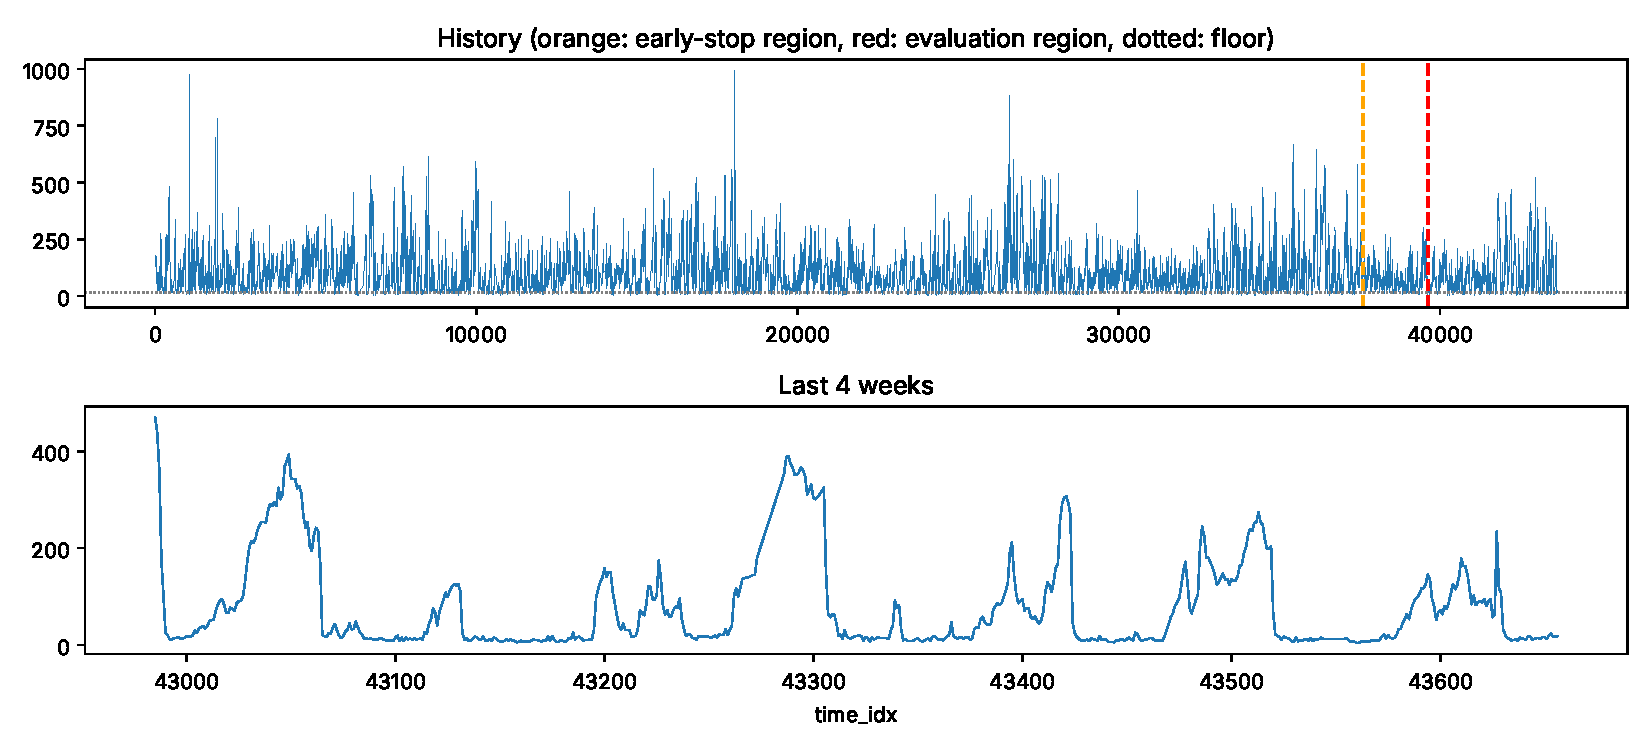
\includegraphics[width=0.95\linewidth]{figures/t2-series.pdf}
\caption{Task 2 history with the early-stop (orange) and evaluation (red) regions; the dotted line is the forecast floor (14.7).}
\label{fig:t2series}
\end{figure}

\begin{figure}[H]\centering
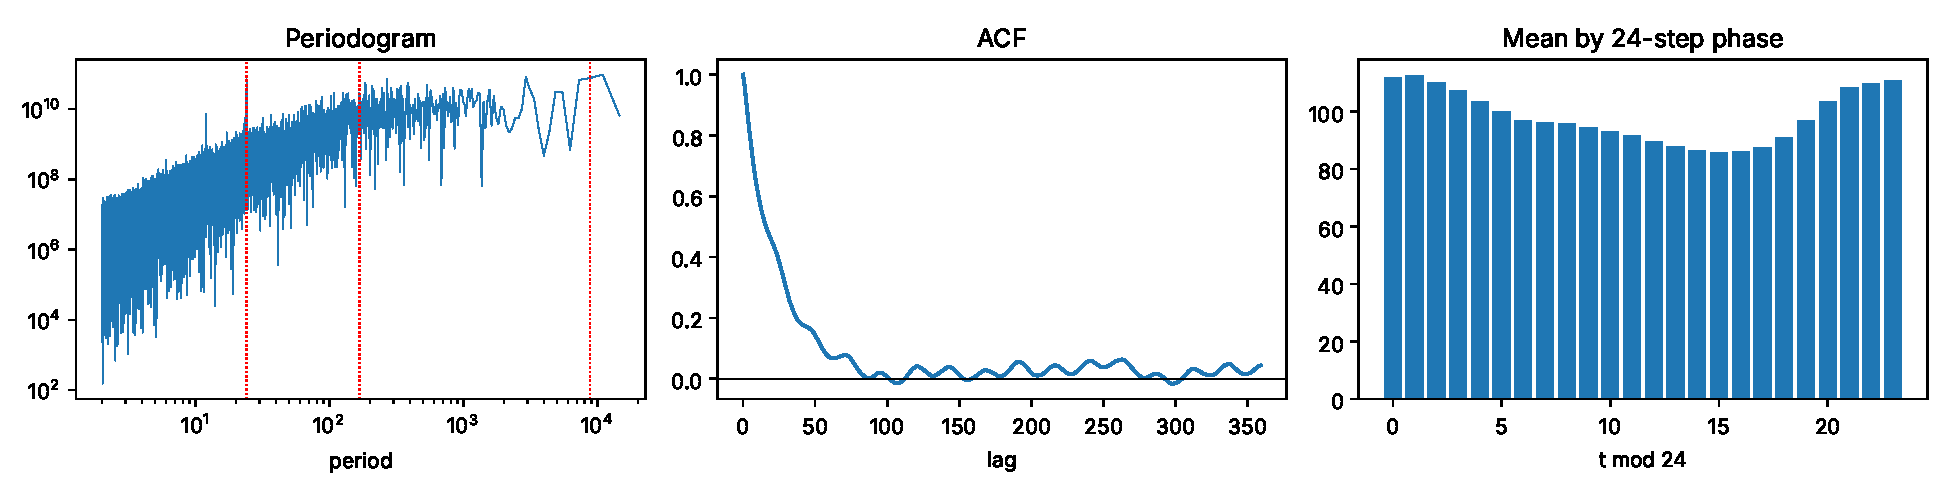
\includegraphics[width=\linewidth]{figures/t2-periodicity.pdf}
\caption{Periodogram, autocorrelation and mean by 24-step phase.}
\label{fig:t2period}
\end{figure}

\begin{itemize}
  \item \textbf{Recovered periods.} The periodogram peaks at \textbf{24} steps and near \textbf{8{,}730} ($\approx$8{,}766), so the sampling interval is most likely hourly, with daily and yearly cycles. The daily cycle is weak: the mean by phase only ranges from 86 to 113 around a mean of 98. Because no calendar is given, I encode these two measured periods as sin/cos ``phase'' features in place of Autoformer's time stamps.
  \item \textbf{Short memory.} The ACF is 0.97 at lag 1, 0.40 at lag 24, 0.16 at lag 48 and 0.03 at lag 168. The recent past says little about most of a 168-step horizon.
  \item \textbf{Heavy tails.} Values range from 0 to 994 and change by an order of magnitude within days. Exact zeros are essentially absent (2 of 43{,}656 hours).
  \item \textbf{External file.} Six continuous features (A--F) and four mutually exclusive flags (G--J). Level correlations with the target are weak (D $-0.25$, H $-0.21$, A $+0.17$, J $+0.15$) and first-difference correlations are near zero, so whether they help had to be settled experimentally. I apply \texttt{log1p} to the heavy-tailed counters D--F, standardise the continuous features on the training region, and keep the flags as 0/1.
\end{itemize}

% ---------------------------------------------------------------------
\subsection*{Validation protocol}

\begin{itemize}
  \item \textbf{Chronological split:} train on steps 1--37{,}608; early stopping only on the next 12 weeks (37{,}609--39{,}624); evaluation on the final \textbf{24 non-overlapping 168-step weeks} (39{,}625--43{,}656), which are never used for fitting or stopping.
  \item \textbf{Metrics:} MAE, RMSE and sMAPE are computed per 168-step week (one leaderboard-sized score each) and averaged over weeks. Weeks 12--23 are the most recent and most volatile, and serve as the closest analogue of the leaderboard week.
  \item \textbf{Seeds:} every configuration uses 3 seeds and is reported as mean $\pm$ std. Differences between configurations are also tested per week (paired, with a 95\% CI over the 24 weeks).
\end{itemize}

\begin{table}[H]\centering\small
\caption{Naive baselines on the 24 evaluation weeks.}
\label{tab:t2base}
\begin{tabular}{lccc}
\toprule
Baseline & MAE & RMSE & sMAPE (\%)\\
\midrule
Persistence (last value) & 96.7 & 117.4 & 89.1\\
Seasonal naive (repeat last 24) & 85.5 & 108.2 & 95.3\\
Mean of last 168 & 68.5 & 83.2 & 80.0\\
Training mean (flat line) & 69.0 & 82.9 & 81.0\\
\bottomrule
\end{tabular}
\end{table}
\noindent Over 168 steps a flat line beats persistence by 34 RMSE, which is consistent with the short memory above. Any model has to beat $\approx$83.

% ---------------------------------------------------------------------
\subsection*{Model design}

\begin{itemize}
  \item \textbf{Autoformer body.} The Auto-Correlation and series-decomposition layers are taken from the official implementation (\href{https://github.com/thuml/Autoformer}{thuml/Autoformer}, MIT licence; Wu et al., 2021), and I wire them as in its reference model: input decomposition (moving average, kernel 25); a decoder trend initialised from the window mean and a seasonal part from zeros; Auto-Correlation in the encoder and in both decoder attentions, keeping $k=\lfloor \ln L\rfloor = 5$ delays; decomposition after every attention and feed-forward block, with the trend accumulated through the decoder.
  \item \textbf{Size:} $d_{\text{model}}=32$, 4 heads, 1 encoder and 1 decoder layer, $d_{ff}=64$. Input length 168, label length 48, \texttt{pred\_len} 168.
  \item \textbf{Embedding (my own):} a circular-conv value embedding plus a linear map of the marks (phase features + covariates), with no positional encoding. The encoder and decoder take separate marks, which is what the external-data ablation varies.
  \item \textbf{Exogenous head:} a term added at each forecast step, computed from the decoder marks over the horizon. Auto-Correlation aggregates time-shifted copies of the whole sequence, which blurs an effect tied to one step, and the head keeps that effect local. It is a 5-step convolution, a GELU and a 1$\times$1 convolution (1{,}153 parameters), so it reacts to \emph{changes} in the covariates, not only their levels.
  \item \textbf{Floor layer:} the last operation is $\max(\hat y, f)$ with $f=14.7$, the 10th percentile of the training target. It has no parameters (see below).
  \item \textbf{Training:} MSE on the standardised target; AdamW (weight decay $10^{-4}$, learning rate $3\times10^{-4}$, $3\times10^{-3}$ for the head); cosine schedule; dropout 0.25; batch 64; training windows every 2 steps; early stopping with patience 4 (maximum 15 epochs).
\end{itemize}
Per model: \textbf{23{,}362} trainable parameters (22{,}209 body and embeddings + 1{,}153 head + 0 floor).

% ---------------------------------------------------------------------
\subsection*{External-data ablation (final model, 3 seeds)}

\begin{table}[H]\centering\small
\caption{With vs.\ without the optional file: mean $\pm$ std over 3 seeds, 24 evaluation weeks.}
\label{tab:t2abl}
\begin{tabular}{lccc}
\toprule
Configuration & MAE & RMSE & sMAPE (\%)\\
\midrule
Target only & 68.2 $\pm$ 2.2 & 82.5 $\pm$ 1.7 & 78.9 $\pm$ 0.9\\
+ external (past only, encoder) & 68.9 $\pm$ 2.4 & 82.8 $\pm$ 1.4 & 79.4 $\pm$ 1.1\\
+ external (past + horizon, encoder and decoder) & \textbf{42.0 $\pm$ 2.4} & \textbf{56.8 $\pm$ 3.0} & \textbf{52.0 $\pm$ 0.3}\\
\bottomrule
\end{tabular}
\end{table}

\begin{figure}[H]\centering
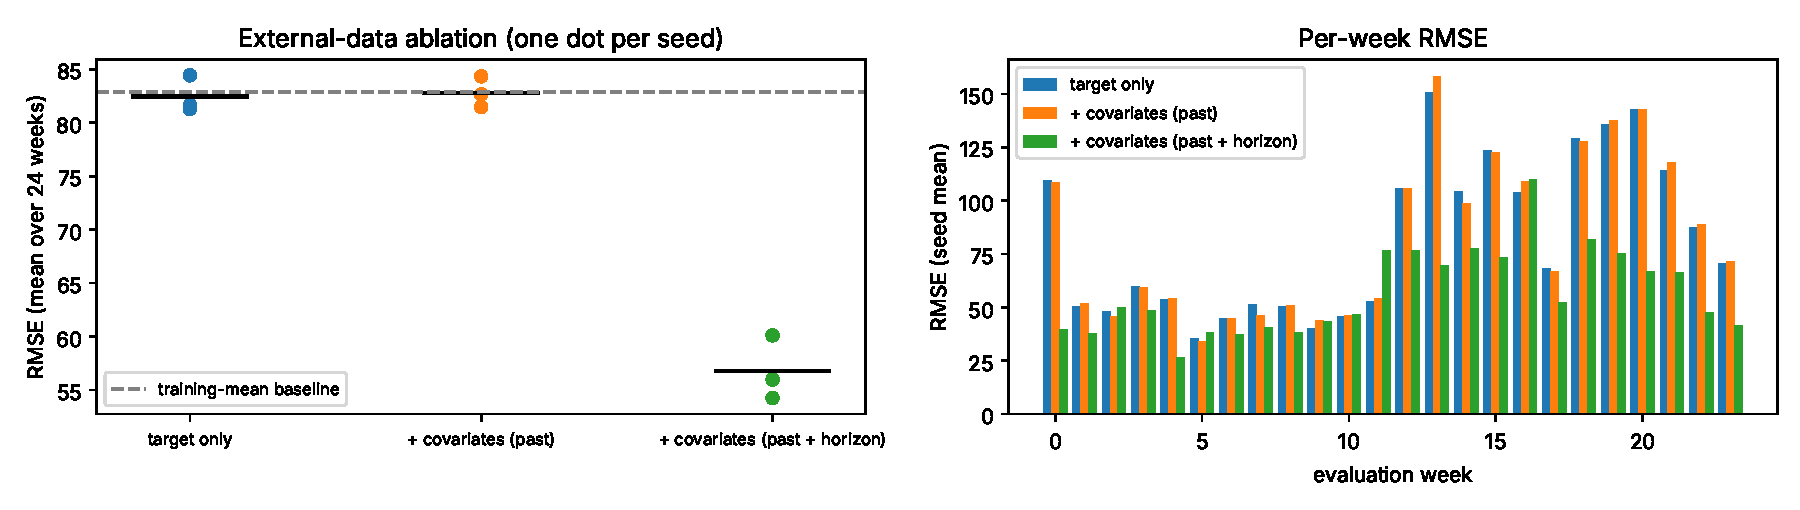
\includegraphics[width=\linewidth]{figures/t2-ablation.pdf}
\caption{External-data ablation: RMSE per seed (left) and per evaluation week (right).}
\label{fig:t2abl}
\end{figure}

\begin{itemize}
  \item \textbf{Covariates help only when they cover the horizon.} Past + horizon vs.\ target only: $\Delta$RMSE $=-25.7 \pm 11.3$, better on 18/24 weeks. Past only vs.\ target only: $+0.4 \pm 1.2$, better on 10/24, i.e.\ no effect.
  \item \textbf{Interpretation.} The covariates are measured on the same clock as the target and are known over the forecast window. Knowing them up to the forecast origin adds nothing, because the target's own memory is short. Their value lies in describing conditions \emph{during} the horizon, so they must enter the decoder.
  \item Without the horizon covariates, the Autoformer is no better than a flat line (82.5 vs.\ 82.9).
\end{itemize}

% ---------------------------------------------------------------------
\subsection*{Submissions and design changes}

Each change below was decided on the evaluation weeks before submitting; the leaderboard was used only to confirm.

\begin{table}[H]\centering\small
\caption{The three leaderboard submissions. Validation = RMSE over the 24 evaluation weeks (all / weeks 12--23) of exactly the configuration submitted.}
\label{tab:t2subs}
\begin{tabular}{clccccc}
\toprule
\# & Model & Val.\ all & Val.\ 12--23 & $P$ & $E$ & Leaderboard RMSE (rank)\\
\midrule
1 & Linear head, 1 seed, no refit, clip at 0 & 63.8 & 79.3 & 22{,}224 & 4 & 93.82 ($\sim$23rd)\\
2 & Non-linear head, 3 seeds + refit, floor after prediction & 56.0 & 71.4 & 70{,}086 & 18 & 71.48 (8th)\\
3 & Non-linear head, 3 seeds + refit, \textbf{floor layer} & \textbf{54.3} & \textbf{68.3} & 70{,}086 & 18 & \textbf{67.22 (3rd)}\\
\bottomrule
\end{tabular}
\end{table}

\begin{table}[H]\centering\small
\caption{Design checks on the past + horizon configuration (3 seeds, RMSE mean $\pm$ std over seeds).}
\label{tab:t2design}
\begin{tabular}{lcc}
\toprule
Configuration & All 24 weeks & Weeks 12--23\\
\midrule
Linear head, dropout 0.1, LR halved each epoch (submission 1) & 60.50 $\pm$ 2.48 & 75.87 $\pm$ 2.43\\
Linear head, dropout 0.25, weight decay, cosine LR & 61.17 $\pm$ 2.11 & 76.20 $\pm$ 2.46\\
Non-linear head, clipped at 0 & 58.12 $\pm$ 2.37 & 72.72 $\pm$ 2.40\\
Non-linear head, floored after prediction (submission 2) & 57.85 $\pm$ 2.42 & 72.58 $\pm$ 2.43\\
Non-linear head, floor layer (submission 3) & \textbf{56.77 $\pm$ 2.46} & \textbf{69.89 $\pm$ 2.37}\\
\midrule
Linear head + 12 more recent weeks in training (refit check) & 59.97 $\pm$ 2.39 & 75.16 $\pm$ 2.37\\
\bottomrule
\end{tabular}
\end{table}

\begin{itemize}
  \item \textbf{Submission 1} scored 93.8 against a validation mean of 60.5. The calm early weeks had flattered the average: on the recent weeks the same model scored 79.3, with weekly RMSE ranging from 33 to 101. From then on I selected on weeks 12--23.
  \item \textbf{Regularisation did not help} ($+0.67 \pm 1.36$, better on 6/24 weeks). Every run still peaked at epoch 1 or 2, so the early stop was not driven by memorisation. Training and recent periods differ, and the covariate head learns the simple signal within one epoch.
  \item \textbf{Non-linear covariate head:} $-3.05 \pm 4.41$ vs.\ the linear head, better on 17/24 weeks. The large errors occur at sudden changes, which a 5-step convolution can represent.
  \item \textbf{Refit and seed averaging.} Training on 12 more recent weeks improved every seed ($-0.53$ RMSE), so the final models are refit on the full history. Averaging the 3 seeds lowers RMSE by a further 1.5--2.5.
  \item \textbf{Floor layer:} $-1.08 \pm 2.63$ RMSE vs.\ the post-hoc floor, but $-3.1$ on the seed-averaged recent weeks (71.40 $\to$ 68.34), and MAE 45.7 $\to$ 42.0.
  \item \textbf{Calibration.} The recent-week validation estimate predicted submissions 2 and 3 to within about one point (71.4 vs.\ 71.48; 68.3 vs.\ 67.22). Submission~1's larger gap is explained by having selected on all 24 weeks.
\end{itemize}

% ---------------------------------------------------------------------
\subsection*{The forecast floor}

\begin{itemize}
  \item \textbf{Why a floor.} The target is non-negative and effectively never zero. Clipping negative outputs at 0 (submission 1) produced runs of exact zeros, whereas on validation weeks where the raw output was negative the truth averaged 14. I therefore use the 10th percentile of the training target, 14.7, fixed from training data only. This is post-hoc truncation to the plausible range; a log or scaled-logit transform (Hyndman \& Athanasopoulos, FPP3 \S13.3) would build the constraint into the model instead.
  \item \textbf{After prediction vs.\ inside the network.} The same $\max(\hat y, 14.7)$ gives different forecasts. Applied after prediction (submission 2), it trims a model that was trained without it and had learned realistic low values (raw outputs mostly between $-20$ and 50 in the low periods of this forecast). Applied as a layer during training (submission 3), it changes what the model learns. The two submissions differ by 18 RMSE.
  \item \textbf{Repeated values of 14.70.} The final forecast sits exactly at 14.70 for 44 of 168 hours (the first 16 and the last 26). In these hours the covariates show the pattern that historically means low values (high C, accumulating D, flag H; hours with this pattern averaged 23, median 16), and all three seeds are clamped. Underneath, the raw outputs are $-35$ to $-390$: because $\partial \max(\hat y, f)/\partial \hat y = 0$ below the floor, no gradient pulls them back, so the model can only say ``at the floor''. This is a limitation, although validation favours it, and a flat 14.70 everywhere would be far worse (RMSE 104.5).
  \item \textbf{Why $P$ and $E$ are identical for submissions 2 and 3.} The floor layer stores 14.7 as a constant, not a trainable weight, so both use $3 \times 23{,}362 = 70{,}086$ parameters. In both, every seed's best early-stopping epoch was 1, with 5 epochs run, giving $E = 3 \times (5 + 1) = 18$.
  \item \textbf{The floor could also be learned.} A learnable floor level (1 parameter per model) would let training choose the level instead of the 10th-percentile rule. A smooth floor ($f + \mathrm{softplus}(\hat y - f)$) would keep a gradient below the floor, so the model could predict, say, 18 or 25 in low periods instead of a flat 14.70. I left both untested: the expected gain was small, the last submission replaces the score, and submission~3 already matched its validation estimate. They are the first next step.
\end{itemize}

% ---------------------------------------------------------------------
\subsection*{Final model: validation and forecast}

\begin{table}[H]\centering\small
\caption{Final model on the 24 evaluation weeks.}
\label{tab:t2final}
\begin{tabular}{lcccccc}
\toprule
Seed & MAE & RMSE & sMAPE (\%) & RMSE weeks 12--23 & Best epoch & Epochs run\\
\midrule
0 & 44.52 & 60.10 & 51.74 & 72.89 & 1 & 5\\
1 & 41.63 & 55.98 & 51.93 & 69.72 & 1 & 5\\
2 & 39.80 & 54.24 & 52.28 & 67.08 & 1 & 5\\
\textbf{3-seed average} & \textbf{40.01} & \textbf{54.26} & \textbf{49.32} & \textbf{68.34} & -- & --\\
\bottomrule
\end{tabular}
\end{table}

\begin{figure}[H]\centering
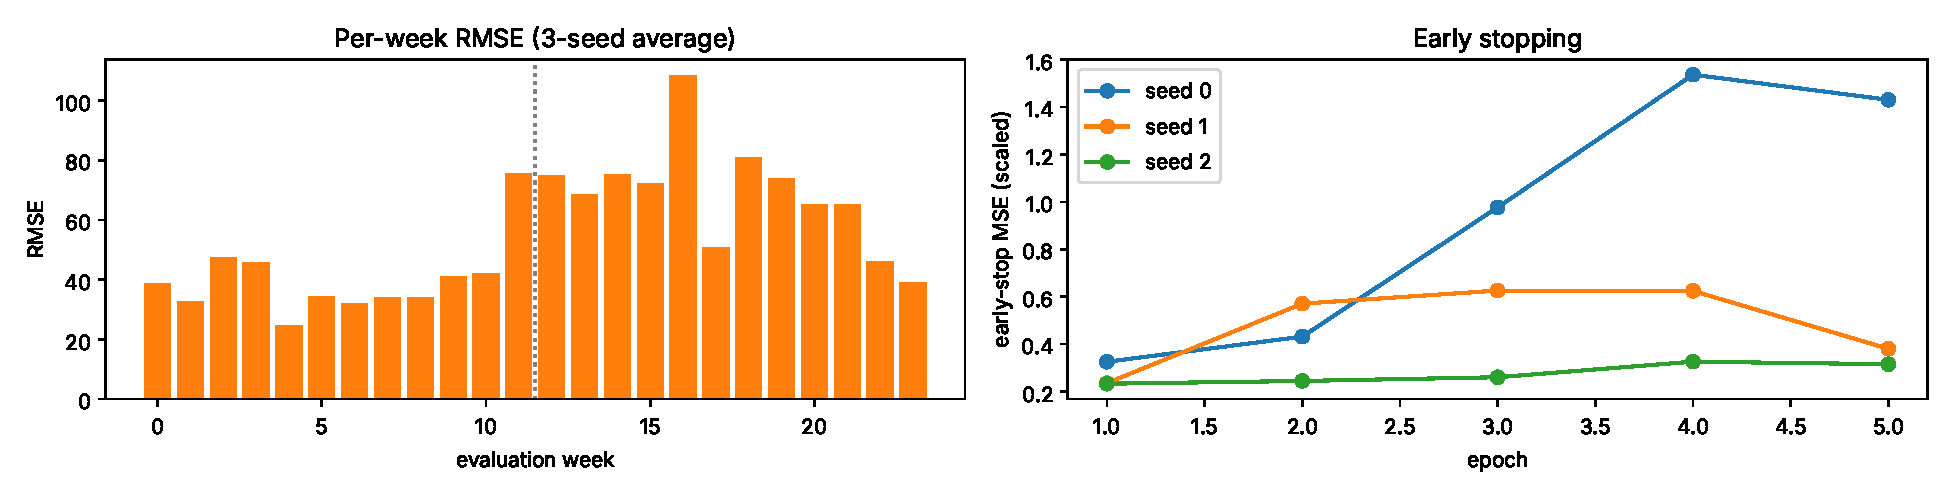
\includegraphics[width=\linewidth]{figures/t2-validation.pdf}
\caption{Final model: per-week RMSE of the 3-seed average (left); early-stopping loss per seed (right).}
\label{fig:t2val}
\end{figure}

\begin{figure}[H]\centering
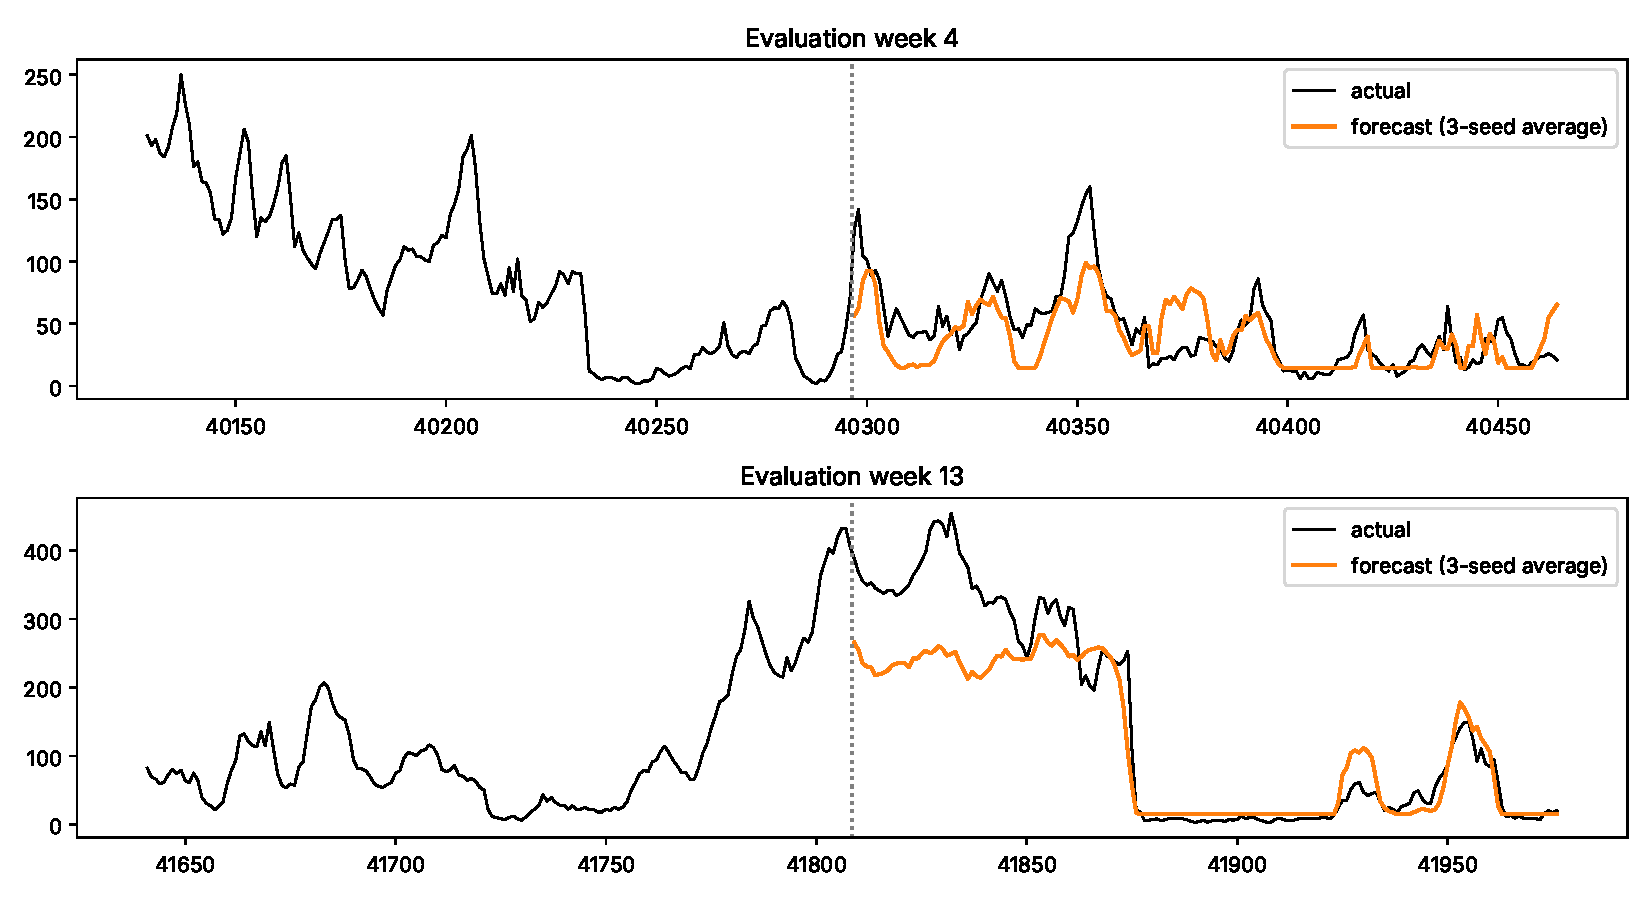
\includegraphics[width=0.95\linewidth]{figures/t2-example-weeks.pdf}
\caption{Two evaluation weeks: actual vs.\ the 3-seed average forecast.}
\label{fig:t2weeks}
\end{figure}

\begin{figure}[H]\centering
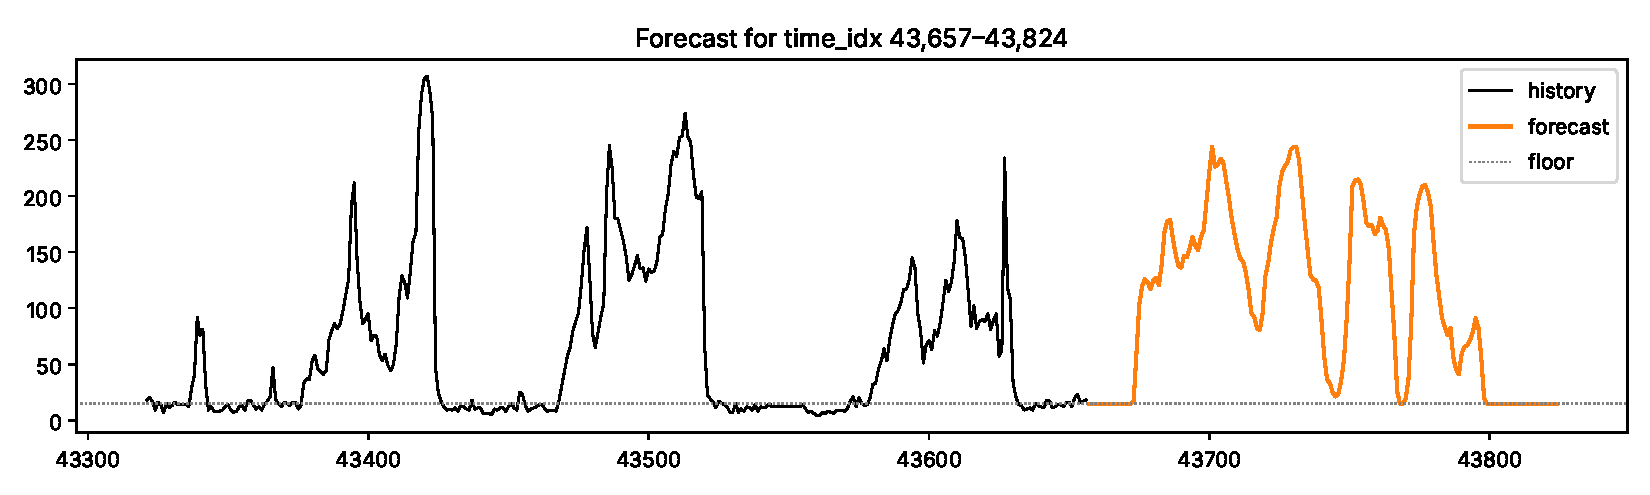
\includegraphics[width=0.95\linewidth]{figures/t2-forecast.pdf}
\caption{Submitted forecast for \texttt{time\_idx} 43{,}657--43{,}824.}
\label{fig:t2fc}
\end{figure}

\begin{infobox}{Final submission (third attempt)}
Each seed is refit on all 43{,}656 steps for its early-stopped epoch count (1), and the three forecasts are averaged.
$P = 3 \times 23{,}362 = \mathbf{70{,}086}$; $E = \sum_{\text{seeds}}(\text{early-stopping epochs run} + \text{refit epochs}) = 3 \times (5+1) = \mathbf{18}$.
Leaderboard: MAE 46.22, \textbf{RMSE 67.22}, sMAPE 42.79\%, score 67.225, \textbf{rank 3}.
\end{infobox}

\paragraph{Limitations.} Early stopping chose epoch 1 in every run, so the Autoformer body adds less than its size suggests; the covariate head carries much of the gain, consistent with Zeng et al.\ (2023). A plain ridge regression on the horizon covariates reached RMSE 57.3 on the same weeks, close to the final model's 54.3.


% =====================================================================
\clearpage
\appendix
\section*{Appendix -- Use of Generative AI}
\addcontentsline{toc}{section}{Appendix: Generative AI use}

\noindent Tool: Claude (Anthropic). For each use: the prompt, the output, and the edits I made.

\begin{enumerate}
  \item \textbf{Prompt:} ``help me understand the assignment, and how i need to solve it'' \\
        \textbf{Output:} overview of Tasks 1--2 and a plan. \\
        \textbf{Edits:} \todo{...}
  \item \textbf{Prompt:} ``write me the code now full for forward'' \\
        \textbf{Output:} the 5-line \texttt{RawAttentionForecaster.forward} assembly. \\
        \textbf{Edits:} \todo{...}
  \item \textbf{Prompt:} ``do it'' (report skeleton) \\
        \textbf{Output:} this \LaTeX\ template (structure and placeholders only). \\
        \textbf{Edits:} \todo{...}
  \item \textbf{Prompt:} ``help me write it'' (\texttt{SeriesDecomposition.forward}, \texttt{aggregate\_delays}) \\
        \textbf{Output:} implementations of both functions (replicate padding + \texttt{avg\_pool1d}; index arithmetic + \texttt{gather}). \\
        \textbf{Edits:} \todo{...}
  \item \textbf{Prompt:} ``help me write the responses seeing the results'' \\
        \textbf{Output:} draft text for Responses 1A (measurement and revision), 1B, 2, 3 and 4(b)--(c), filled tables and figure placement, based on my full-run outputs. My predictions in 1A and 4(a) and my deployment choices were my own. \\
        \textbf{Edits:} \todo{describe what you changed}
  \item \textbf{Prompt:} ``alright go with 2, but guide me over what's being done'' (Task 2) \\
        \textbf{Output:} data exploration, the validation protocol, the Autoformer pipeline (cited thuml layers, my own embedding wiring) and the three-variant external-data ablation, with step-by-step explanations. \\
        \textbf{Edits:} \todo{...}
  \item \textbf{Prompt:} ``isn't the model performing very low?'' / ``what changes do you suggest\ldots'' \\
        \textbf{Output:} a comparison against a ridge yardstick and the published Autoformer results, and the proposals tested here (regularisation, refit, seed averaging, non-linear covariate head). \\
        \textbf{Edits:} \todo{...}
  \item \textbf{Prompt:} ``why can't we do something in training that improves that?'' / ``apply that max within the layer'' \\
        \textbf{Output:} the floor analysis and the floor layer (submission 3), its validation, and the standalone \texttt{Task2\_v4.ipynb}. \\
        \textbf{Edits:} \todo{...}
  \item \textbf{Prompt:} ``create a report now based on what we did in first, second and third\ldots'' \\
        \textbf{Output:} draft text, tables and figures for the Task 2 section of this report, from my runs and leaderboard results. \\
        \textbf{Edits:} \todo{describe what you changed}
\end{enumerate}

\end{document}
